%
% ======================================================================
\RequirePackage{docswitch}
% \flag is set by the user, through the makefile:
%    make note
%    make apj
% etc.
\setjournal{\flag}

\documentclass[\docopts]{\docclass}

% You could also define the document class directly
%\documentclass[]{emulateapj}

% Custom commands from LSST DESC, see texmf/styles/lsstdesc_macros.sty
\usepackage{lsstdesc_macros}

\usepackage{graphicx}
\graphicspath{{./}{./figures/}}
\bibliographystyle{apj}

% Add your own macros here:



%
% ======================================================================

\begin{document}

\title{ The LSST DESC Data Challenge 1: Simulating data for the next generation of photometric redshift surveys }

\maketitlepre

\begin{abstract}

The success of future Stage IV dark energy surveys~\citep{2006astro.ph..9591A} relies in the ability to model and mitigate
systematic uncertainties. Realistic simulation offer a unique opportunity to study systematic uncertainties and test the
processing and analysis pipelines of ongoing and future experiments. Here we present a set of realistic simulations
of $\sim 40$ sq.-deg. that try to mimic the depth and characteristics of LSST 10-years coadd images in the $r$-band.
We characterize our samples performing several astrometric and photometric checks to assess the quality of the
measurements and to enable the usage of these simulations for future studies.

\end{abstract}

% Keywords are ignored in the LSST DESC Note style:
\dockeys{latex: templates, papers: awesome}

\maketitlepost

% ----------------------------------------------------------------------
%

\section{Introduction}
\label{sec:intro}

The increase in statistical power from recent cosmological experiments makes the modeling, and mitigation of systematic
uncertainties key to extract the maximum performance and produce competitive analyses. More traditional in high energy
particle physics~\citep{Brun:118715},~\citep{2006JHEP...05..026S}, end-to-end simulations provide a unique framework to
model systematics and streamline processing and analysis pipelines given that we have complete information about the inputs
and outputs. With the larger availability of computational resources this approach has also been extended to photometric
redshift galaxy surveys~\citep{2016MNRAS.457..786S,2016ApJ...817...25B} and a similar effort is undergoing in spectroscopic
surveys such as DESI~\citep{2016arXiv161100036D}. For surveys like the LSST~\citep{2008arXiv0805.2366I} where the expected
data volume is very large and where a highly stringent control of the systematic uncertainties is required, producing these
kind of end-to-end simulations becomes necessary.

In this paper, we present the procedure to generate and process images that resemble the data that will be produced by
LSST~\citep{2008arXiv0805.2366I} after 10 years of operation in $r$-band using state of the art tools. We also characterize
the products of this process for future studies. These productsencompass single-visit and coadded calibrated exposures
(i.e., flattened, background removed, etc) and source catalogs that add up to $\sim 225 TB$. They are the result of three
different simulations: imSim dithered, imSim undithered, and PhoSim that will be introduced later.

This paper is structured as follows: In \secref{inputs} we describe the input catalog used for our simulations,
in \secref{image_generation_pipeline} we introduce two different approaches to generate simulated images to
resemble LSST data. In \secref{image_processing_pipeline} we present the procedure and tools used to perform
calibration and source extraction on the simulated images. In \secref{catalogs} we describe the output catalogs
produced by our pipelines. Finally, in \secref{conclusions} we present some concluding remarks.

% ----------------------------------------------------------------------
\section{Image generation: inputs}
\label{sec:inputs}

\textcolor{red}{Describe CatSim inputs and dithering}

\section{Image generation: pipeline}
\label{sec:image_generation_pipeline}
% ---------------------------------------------------------------------

The artificial generation of astronomical images is a very complex and computationally demanding process. In the recent
years there is a big effort in the community in order to create software that allows more realistic and fast image
generation~\citep{2016MNRAS.457..786S,2016ApJ...817...25B}. In our case, we use two different approaches: In one approach
we use modeling of the input sources using \textsc{GalSim}~\citep{2015A&C....10..121R}. The other approach consists in
running a full photon-shooting simulation using \textsc{PhoSim}~\citep{2015ApJS..218...14P}. The former has a big speed
advantage but the latter fully traces each photon coming from the sources through the atmosphere and the instrument,
 increasing the level of realism. These two approaches allow us to focus on different systematic effects and science cases.

\subsection{The imSim pipeline}
\label{sec:imsim_pipeline}

\textcolor{red}{Describe imSim}
% ----------------------------------------------------------------------

\subsection{The PhoSim pipeline}
\label{sec:phosim_pipeline}

\textcolor{red}{Describe PhoSim}
% ----------------------------------------------------------------------

\section{Image processing pipeline}
\label{sec:image_processing_pipeline}

Once the images are produced we process them using the LSST software stack~\citep{2015arXiv151207914J}. This is an open
source high-performance data processing and analysis system intended for use in O/IR survey data. The code can be found at
\url{dm.lsst.org} and \url{pipelines.lsst.io}. The raw, uncalibrated single exposures are used as inputs. The software performs
the reduction, detection, deblending and measurement on individual visits and coadds producing the level 2 data
products~\citep{2015arXiv151207914J}.

\textcolor{red}{Say something about data size, times, configuration, etc}
% ----------------------------------------------------------------------

\section{Output catalogs}
\label{sec:catalogs}

After being processed, the catalogs are accessible by DESC collaborators andstored at NERSC. We generate pandas
dataframes and three different databases for each one of the total coadd catalogs in order to be accessed by the
collaborators and perform their own analyses. These catalogs contain 10.6 million objects covering an area
of $\sim$ 43 deg$^{2}$.

In order to check the level of realism and the accuracy of the processed catalogs we perform several quality assurance tests.
We focus on three different areas that can induce a systematic effect in the weak lensing and clustering observables:
astrometry, photometry and PSF.

\subsection{Astrometry checks}
\label{sec:astrometry_checks}

Biases on astrometry can potentially affect both clustering and weak lensing measurements. These biases
can have different origins: PSF mis-characterization, not corrected sensor effects, presence of blended sources are among
the most common scenarios for single-visit exposures. In the case of co-adds we should add to this list a different effect:
incorrect modeling of proper motion for the measured objects.

We will follow two approaches to check the quality of the astrometric solutions that we obtained: an \textit{external} check
comparing to the input \textit{truth} catalog; and an \textit{internal} check comparing different visits.

\subsubsection{External checks}
\label{sec:external_astrometry}

As we have already mentioned, one of the big advantages of using simulations is that we have access to the \textit{true}
underlying information. We will use this information to check the precision of the astrometric measurements in single exposures
and co-adds. For these and the photometry studies we will select stellar objects. In order to do so, we use the classifier
included in the LSST software stack\footnote{To see more details about the classifier refer to section 4.9.10 at
~\citep{2017arXiv170506766B}} and choose objects with \texttt{base\_ClassificationExtendedness\_value==0}.
We also require that \texttt{deblend\_nChild==0} to ensure that the objects are primary sources. We match these objects to the
stellar source in the input catalog. In both cases we will use a \texttt{KDTree}~\citep{scikit-learn} to retrieve those objects
in the input catalog that are in a radius of 0.2 arc-seconds (one pixel) of those detected in the output catalog and select the
match that is closest in magnitude. We only consider sources which have a magnitude difference smaller than 0.02 magnitudes.

We selected a representative single visit (visit number $270675$ for the imSim dithered run) and calculated the difference
between the measured and the input positions. These are represented in \figref{astrometry_a}. We can see that both RA and Dec
distributions are compatible with each other, meaning that there are no anisotropies in the detection, as expected from the inputs.
However, we find that the distributions are assymetric and that the median is not zero. This effect is even more noticeable when we
accumulate visits as in \figref{astrometry_b}, where we accumulated the results for 50 randomly selected visits of the imSim dithered
run. This effect is also present in the dithered and undithered imSim runs and in the PhoSim run. We also checked the dependence the
mean astrometric residual with the magnitude of the objects as shown in \figref{astrometry_b} where a mild bias for the brightest
objects can be seen. This bias is smaller than 15 mas, much smaller than the resolution of the input N-body simulation. This means
that the two point clustering statistics will not be affected by this bias.
\textcolor{red}{Check origin of these biases: Some pepole suggest proper motion: Why then
present in single visits? I think it's the way we simulate the saturation (see the trend with magnitude).}

\begin{figure}
  \centering
  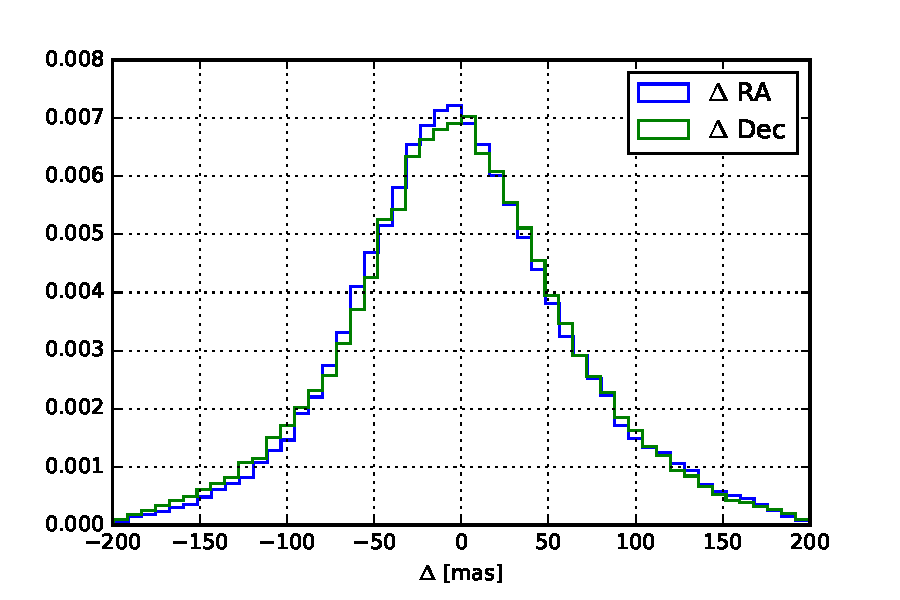
\includegraphics[width=0.45\textwidth]{astrometry_single_visit_imsim_dithered_hist}
  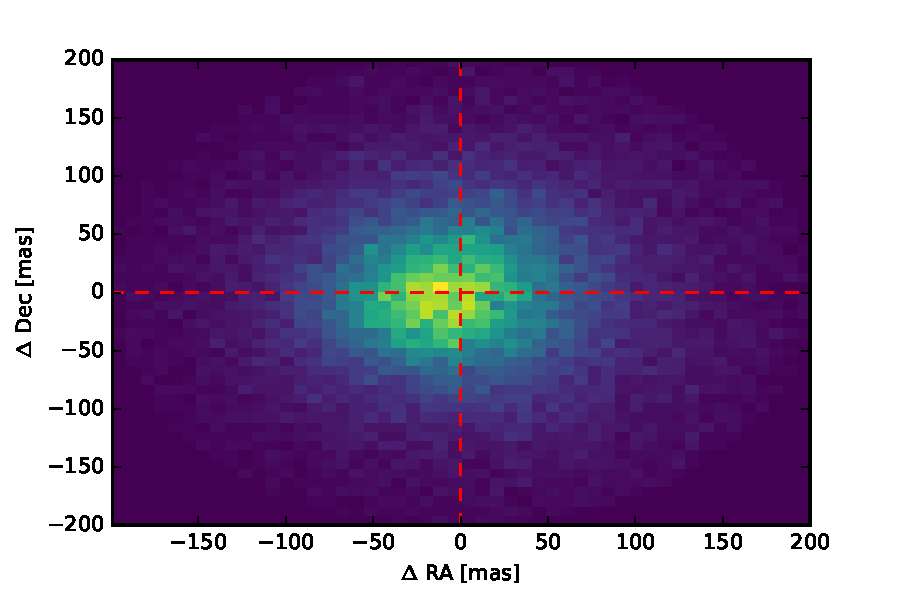
\includegraphics[width=0.45\textwidth]{astrometry_single_visit_imsim_dithered_hist2d}
  \caption{Left: Distribution of the difference $\Delta=X_{measured}-X_{input}$ in RA (blue) and Dec (green) coordinates. We cannot
  appreciate any differences between these, however we see that there is median is not at zero $\Delta_{median} \approx -2$ mas.
  The histograms are normalized such that the total sum of the counts is equal to one. Right: 2D histogram
  showing the bivariate distribution of the difference in RA (horizontal axis) and Dec (vertical axis). We selected one random representative
  exposure (visit number $270675$ for the imSim dithered run). The effect is similar for the undithered imSim run and for the PhoSim run.}
  \label{fig:astrometry_a}
\end{figure}

\begin{figure}
  \centering
  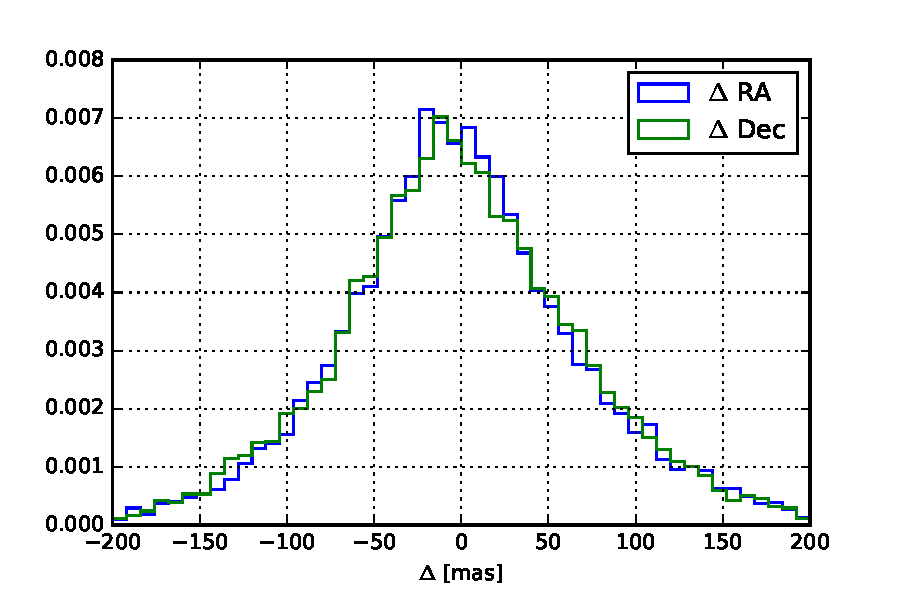
\includegraphics[width=0.3\textwidth]{astrometry_imsim_dithered_50visits}
  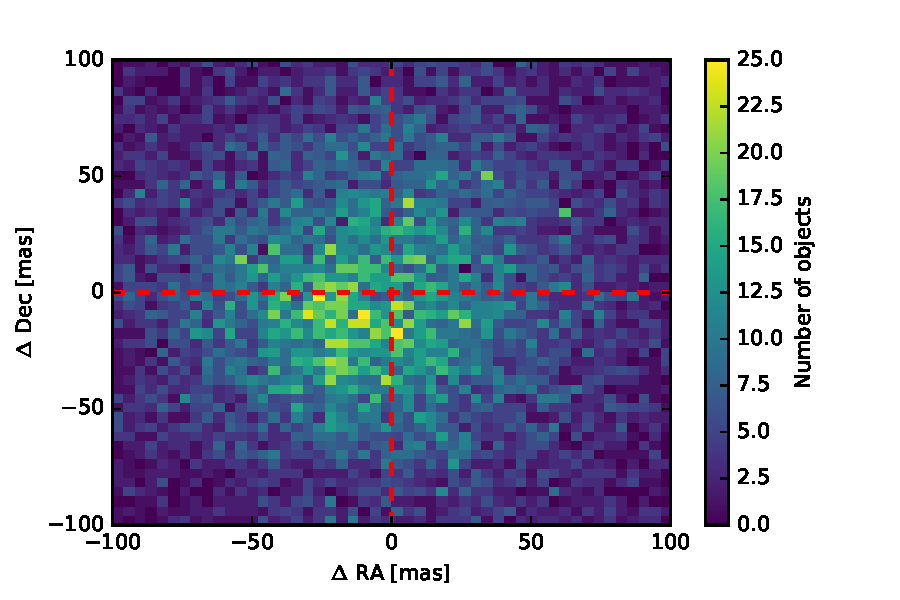
\includegraphics[width=0.3\textwidth]{astrometry_imsim_dithered_50visits_hist2d}
  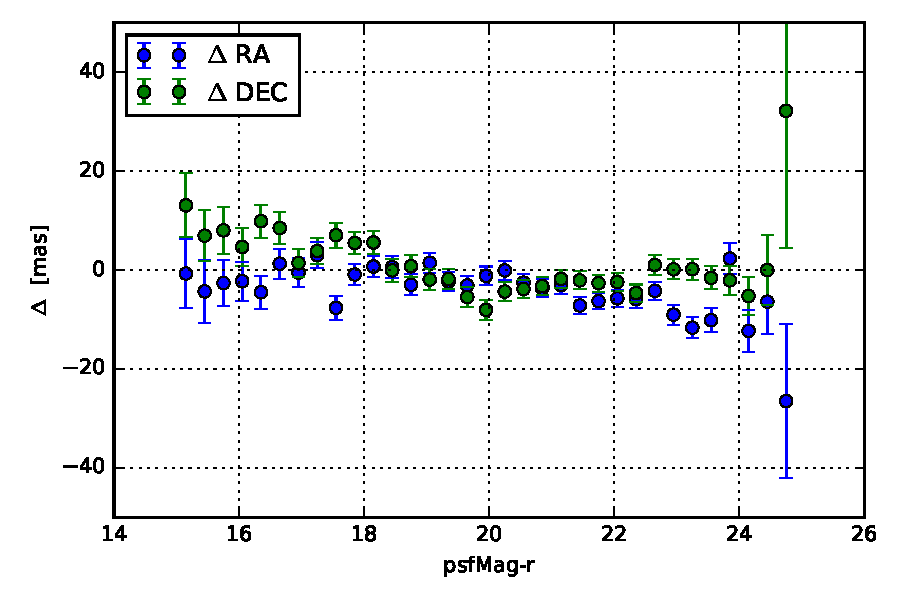
\includegraphics[width=0.3\textwidth]{astrometry_vs_mag_imsim_50_visits}
  \caption{Left: Distribution of the difference $\Delta=X_{measured}-X_{input}$ in RA (blue) and Dec (green) coordinates as in
  \figref{astrometry_a} but accumulating the results for 50 randomly selected visits from the imSim dithered run. Middle: 2D histogram
  showing the bivariate distribution of the difference in RA (horizontal axis) and Dec (vertical axis). Right: Mean astrometric residual
  as a function of magnitude for RA (blue) and Dec (green). These distributions are similar for the undithered imSim run and for the PhoSim run.}
  \label{fig:astrometry_b}
\end{figure}

We also wanted to check if there is a preferred orientation for the differences between the input and output position in a single visit. Using
the same visit as before we show the astrometric residuals in \figref{astrometry_c}. In this Figure we can see that the astrometric
residuals do not show any noticeable structure and appear to be mostly random.

\begin{figure}
  \centering
  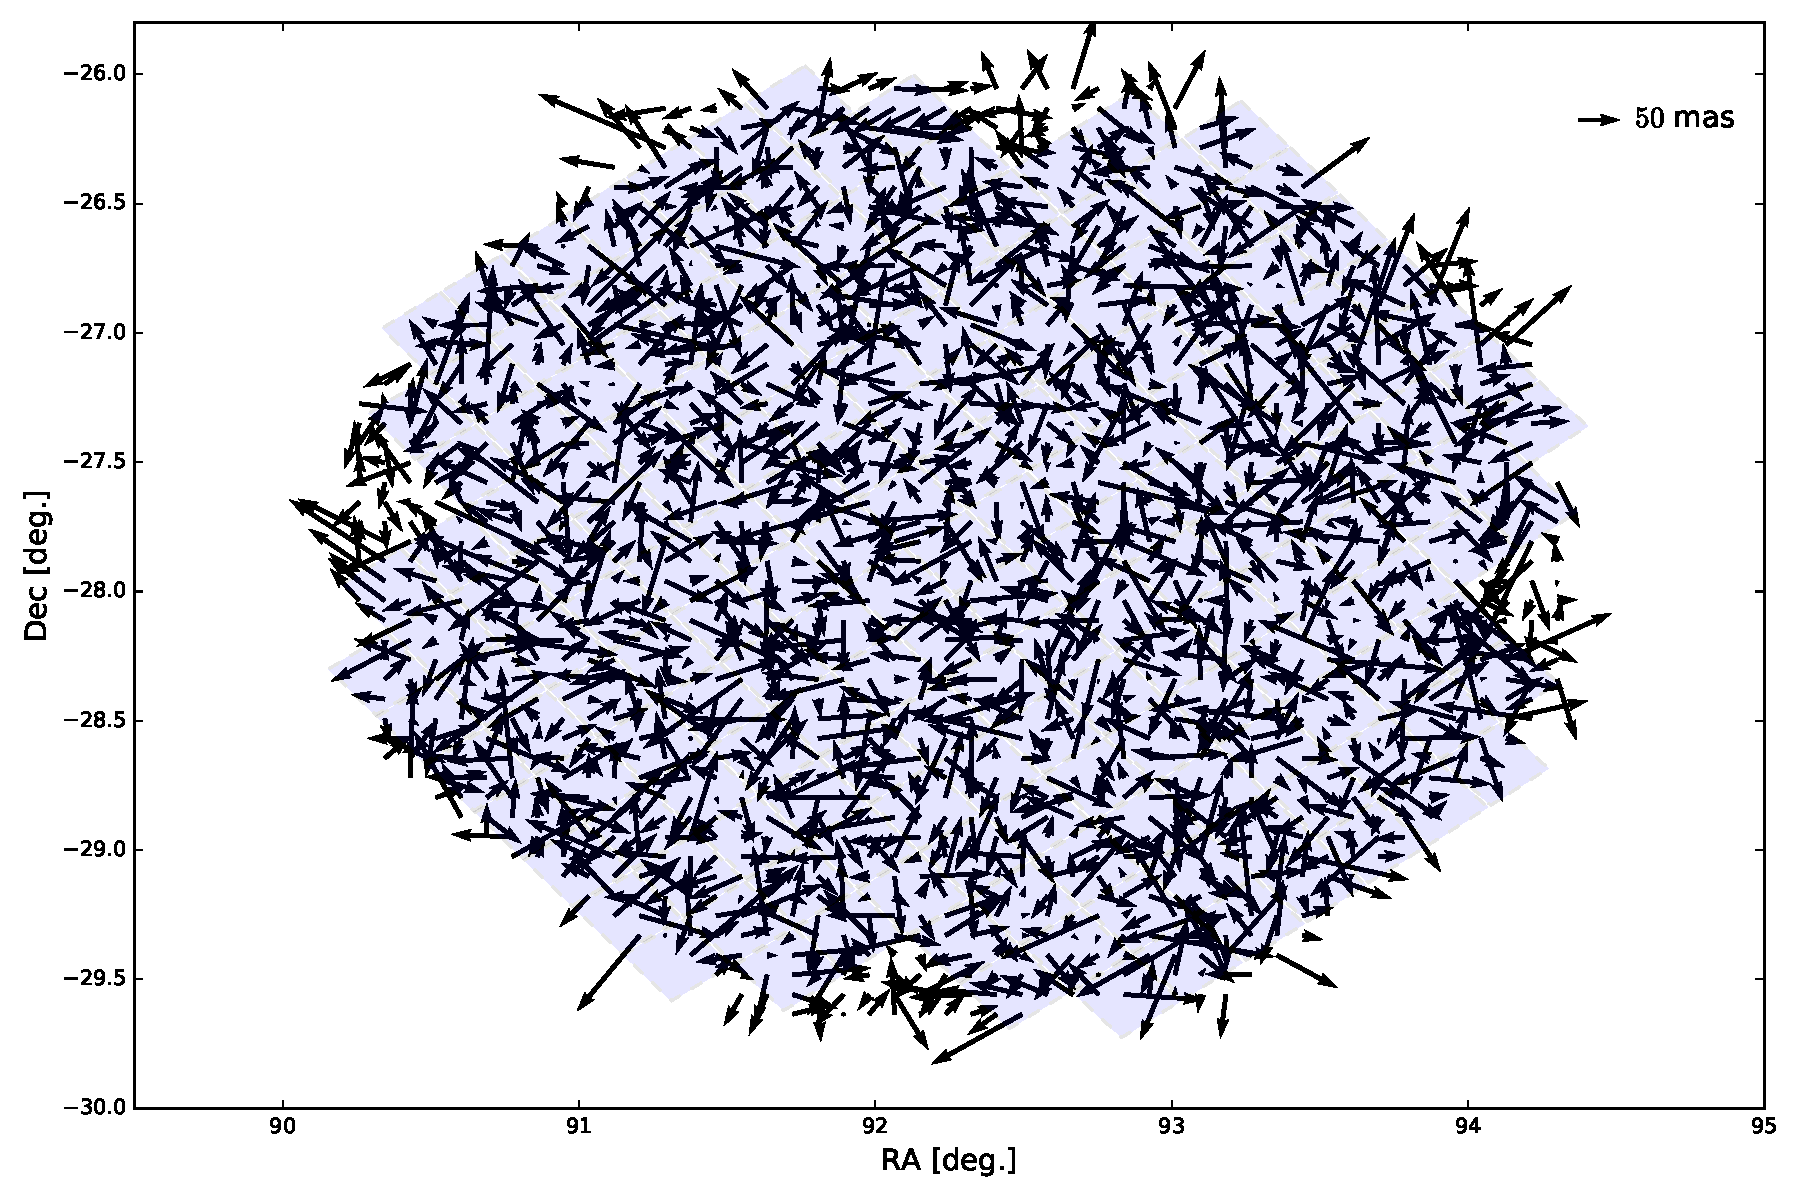
\includegraphics[width=0.7\textwidth]{astrometry_imsim_dithered_interp}
  \caption{Astrometic residuals measured in visit $270675$ from the imSim dithered run. The light blue squares represent the CCD chips in
  the LSST focal plane. The base of the arrow is on the input matched object. The arrows have been re-scaled 10,000 for visualization purposes.}
  \label{fig:astrometry_c}
\end{figure}


\subsubsection{Internal checks}
\label{sec:internal_astrometry}

We also wanted to check the internal consistency of the astrometric solutions between different exposures. To do that we selected a small
region of the co-added area, which we will refer to as \textit{patch} and compared the positions of the objects detected in the co-add
image with the positions of objects detected in individual exposures that overlap with that patch.

In particular, we randomly chose 10 catalogs from individual exposures and looked for objects that fulfilled the following criteria:
\begin{itemize}
  \item \texttt{deblend\_nChild==0}, this means that the object has been completely deblended (it is a primary match).
  \item \texttt{base\_PixelFlags\_flag\_edge==0}, which means that the object is not close to an edge.
  \item \texttt{base\_PixelFlags\_flag\_interpolatedCenter==0}, the object does not have any interpolated pixels in its center.
\end{itemize}
Note that in this case we are not requiring the objects to be clasiffied as stars (we are omitting the cut in
\texttt{base\_ClassificationExtendedness\_value}) but we are adding some cuts to ensure that the objects were properly measured. Once
we perform our selection, the next step is to match the objects in the different exposures. To do so we use the matching algorithm
included in the LSST software stack\textcolor{red}{Reference?} and calculate the mean of the difference between the position of each source
in the co-add, $X_{coadd,i}$ and the position of the matched object in each of the exposures where it has been detected, $X_{visit_{j},i}$
for $j \in [1,10]$, i.e,
\begin{equation}
  \Delta = \langle X_{coadd,i} - X_{visit_{j},i} \rangle
\end{equation}
we only consider sources that have been detected in at least 5 exposures. The resulting distribution is shown in \figref{astrometry_internal}
where we see that is noticeably narrower than those shown in \figref{astrometry_a} and \figref{astrometry_b}.
\begin{figure}
  \centering
  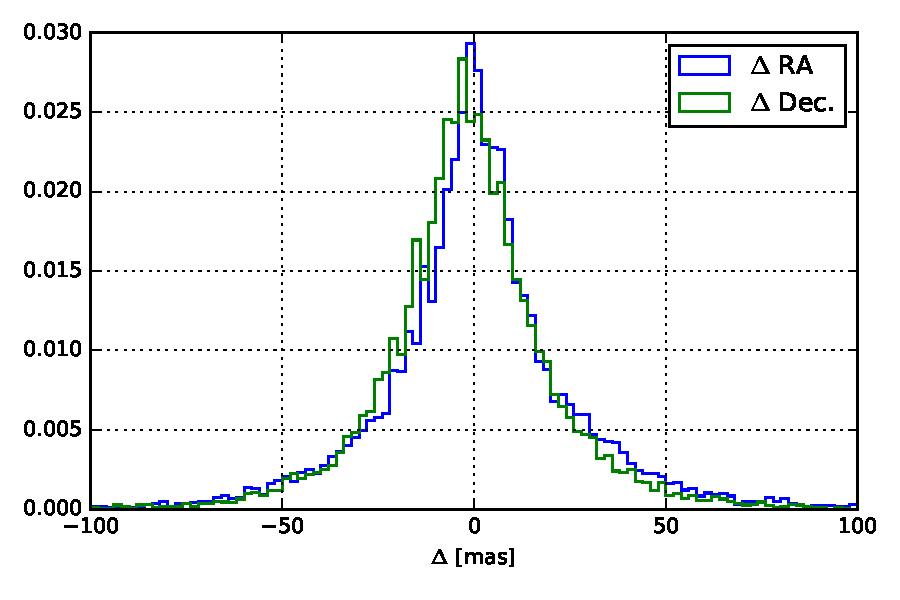
\includegraphics[width=0.45\textwidth]{astrometry_internal_10visits_imsim_undithered}
  \caption{Distribution of the mean difference in position (RA:blue, Dec:green) between the coadd and the different individual exposures
  where each source has been detected.}
  \label{fig:astrometry_internal}
\end{figure}

\subsection{Photometry checks}
\label{sec:photometry_checks}

As in previous sections we are going to perform two different tests to test the quality of our simulations; first we are going to
compare our output catalogs to the inputs, and second we are going to check the consistency between different visits for the same objects.

\subsubsection{External checks}
\label{sec:external_photometry}

For the external checks we use again the same 50 randomly selected visits as we did in the previous section to check the astrometric residuals.
To study the photometric residuals we change slightly the matching strategy from previous sections. In this case we eliminate the threshold
in magnitude difference so, we just look for the input source that is closest in magnitude in a 0.2 arc-seconds radius around each detected
source. In \figref{photometry_a} we can see the distribution of the photometric residuals. We see that this distribution gets wider as we go
fainter (as expected) and that the 0.02 magnitude selection cut was a good proxy to ensure that we account for most sources properly matched.

\begin{figure}
  \centering
  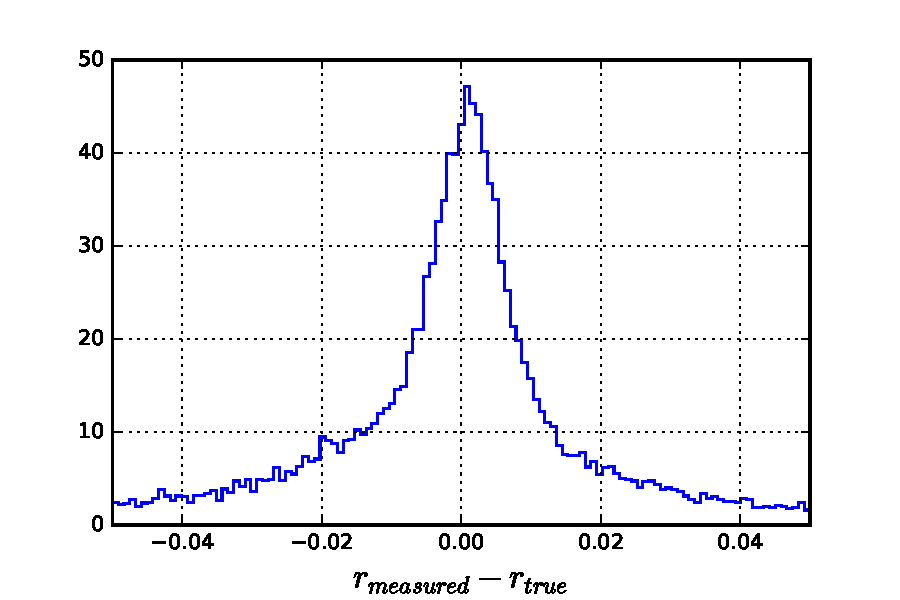
\includegraphics[width=0.45\textwidth]{photometry_imsim_dithered_50visits_hist}
  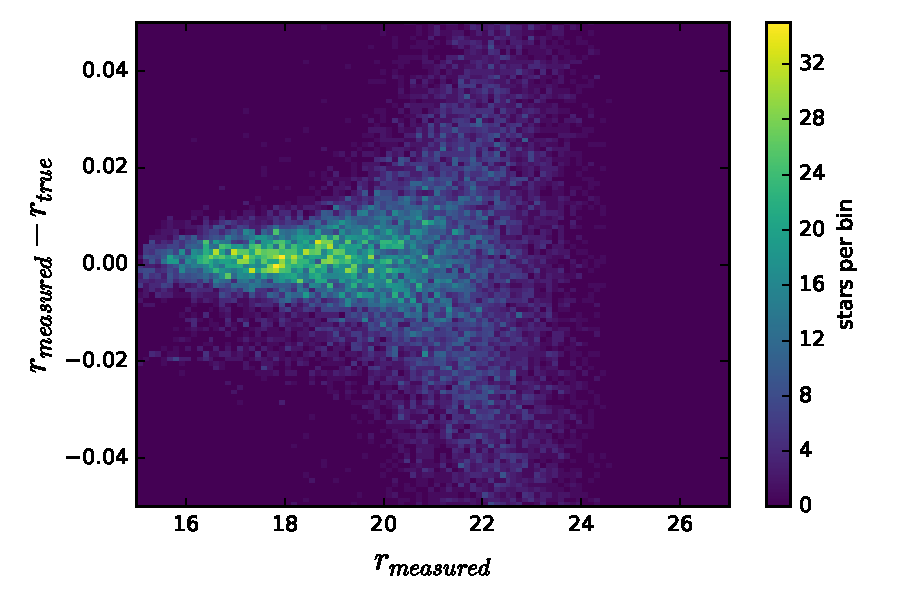
\includegraphics[width=0.45\textwidth]{photometry_imsim_dithered_50visits}
  \caption{Left: Distribution of magnitude difference between the input and output catalogs.
  Right: Difference magnitude between input and output catalogs as a function of the measured magnitude. We considered 50 visits
  randomly selected from the imSim dithered run. We find similar results for the imSim undithered run and for the PhoSim run.}
  \label{fig:photometry_a}
\end{figure}

\subsubsection{Internal checks}
\label{sec:internal_photometry}


\subsection{PSF checks}
\label{sec:psf_checks}

% ----------------------------------------------------------------------

\section{Conclusions}
\label{sec:conclusions}


% ----------------------------------------------------------------------

\subsection*{Acknowledgments}

Here is where you should add your specific acknowledgments, remembering that some standard thanks will be added
via the \code{acknowledgments.tex} and \code{contributions.tex} files.

% 
This is the text imported from \code{acknowledgments.tex}, and will be replaced by some standard LSST DESC boilerplate at some point.
% 


Author contributions are listed below. \\
Yusra AlSayyad: Contribution \\
Humna Awan: Contribution \\
Colin Burke: Contribution \\
Jun Cheng: Contribution \\
James C. Chiang: Contribution \\
Scott Daniel: Contribution \\
Seth Digel: Contribution \\
Richard Dubois: Contribution \\
Eric Gawiser: Contribution \\
Tom Glanzman: Contribution \\
Mike Jarvis: Contribution \\
Tony Johnson: Contribution \\
Heather Kelly: Contribution \\
David Kirkby: Contribution \\
Simon Krughoff: Contribution \\
Robert Lupton: Contribution \\
Rachel Mandelbaum: Contribution \\
P.~Marshall: Contribution \\
Mustafa Mustafa: Contribution \\
En-Hsin Peng: Contribution \\
John Peterson: Contribution \\
Paul Price: Contribution \\
Javier Sanchez: Validation and analysis, started note \\
Glenn Sembroski: Contribution \\
Anze Slosar: Contribution \\
Brian Van Klaveren: Contribution \\
Chris W. Walter: Contribution \\
Matt Wiesener: Contribution \\
Bo Xin: Contribution \\


%{\it Facilities:} \facility{LSST}

% Include both collaboration papers and external citations:
\bibliography{lsstdesc,main}

\end{document}
% ======================================================================
%
